\documentclass[tikz,border=12pt]{standalone}
\usepackage{tikz}
\usepackage{amsmath}
\usepackage{amssymb}
\usetikzlibrary{
  shapes.geometric,
  shapes.multipart,
  arrows.meta,
  positioning,
  fit,
  backgrounds,
  shadows.blur,
  calc,
  matrix,
  decorations.pathreplacing,
  decorations.markings
}

%% ===== COLOR PALETTE =====
\definecolor{CPurple50}{HTML}{EEEDFE}
\definecolor{CPurple400}{HTML}{7D77D4}
\definecolor{CPurple600}{HTML}{534AB7}
\definecolor{CPurple800}{HTML}{3C3489}
\definecolor{CTeal50}{HTML}{E1F5EE}
\definecolor{CTeal400}{HTML}{3CB88A}
\definecolor{CTeal600}{HTML}{0F6E56}
\definecolor{CTeal800}{HTML}{085041}
\definecolor{CAmber50}{HTML}{FAEEDA}
\definecolor{CAmber400}{HTML}{D48B2E}
\definecolor{CAmber600}{HTML}{854F0B}
\definecolor{CCoral50}{HTML}{FAECE7}
\definecolor{CCoral400}{HTML}{D85A30}
\definecolor{CCoral600}{HTML}{993C1D}
\definecolor{CRed50}{HTML}{FCEBEB}
\definecolor{CRed400}{HTML}{C94040}
\definecolor{CRed600}{HTML}{A32D2D}
\definecolor{CGray50}{HTML}{F5F4F0}
\definecolor{CGray200}{HTML}{D8D5C8}
\definecolor{CGray500}{HTML}{888780}
\definecolor{CGray800}{HTML}{444441}
\definecolor{CBlue50}{HTML}{E6F1FB}
\definecolor{CBlue600}{HTML}{185FA5}
\definecolor{CWhite}{HTML}{FFFFFF}

%% ===== TIKZ STYLES =====
\tikzset{
  %% --- State nodes (Kripke) ---
  state/.style={
    circle, draw=CGray500, line width=0.8pt,
    fill=CGray50, text=CGray800,
    font=\small\bfseries,
    minimum size=1.1cm, inner sep=2pt, align=center
  },
  state init/.style={state, double, double distance=1.5pt,
    fill=CTeal50, draw=CTeal600, text=CTeal800},
  state assigned/.style={state,
    fill=CPurple50, draw=CPurple600, text=CPurple800},
  state calc/.style={state,
    fill=CAmber50, draw=CAmber600, text=CAmber600},
  state exported/.style={state,
    fill=CTeal50, draw=CTeal600, text=CTeal800},
  state error/.style={state,
    fill=CRed50, draw=CRed600, text=CRed600},
  state buggy/.style={state,
    fill=CCoral50, draw=CCoral600, text=CCoral600,
    dashed},
  %% --- Arrows ---
  arr/.style={
    -Stealth, line width=0.9pt, color=CGray500
  },
  arr red/.style={
    -Stealth, line width=1.0pt, color=CRed400,
    dashed
  },
  arr teal/.style={
    -Stealth, line width=1.0pt, color=CTeal600
  },
  arr purple/.style={
    -Stealth, line width=1.0pt, color=CPurple600
  },
  arr amber/.style={
    -Stealth, line width=1.0pt, color=CAmber600
  },
  %% --- Labels ---
  edge label/.style={
    font=\scriptsize, text=CGray500,
    fill=CWhite, inner sep=1pt
  },
  title main/.style={font=\large\bfseries, text=CGray800},
  title sub/.style={font=\small, text=CGray500},
  badge/.style={
    rectangle, rounded corners=2pt,
    font=\scriptsize\bfseries,
    inner sep=3pt, minimum height=0.45cm,
    text=CWhite
  }
}

\begin{document}
%% ===========================================================
%% DIAGRAM 1: SƠ ĐỒ CHUYỂN TRẠNG THÁI (STATE TRANSITION)
%% Kripke M = (S, S0, R, L) — 5 states FIXED + S5 BUGGY only
%% ===========================================================
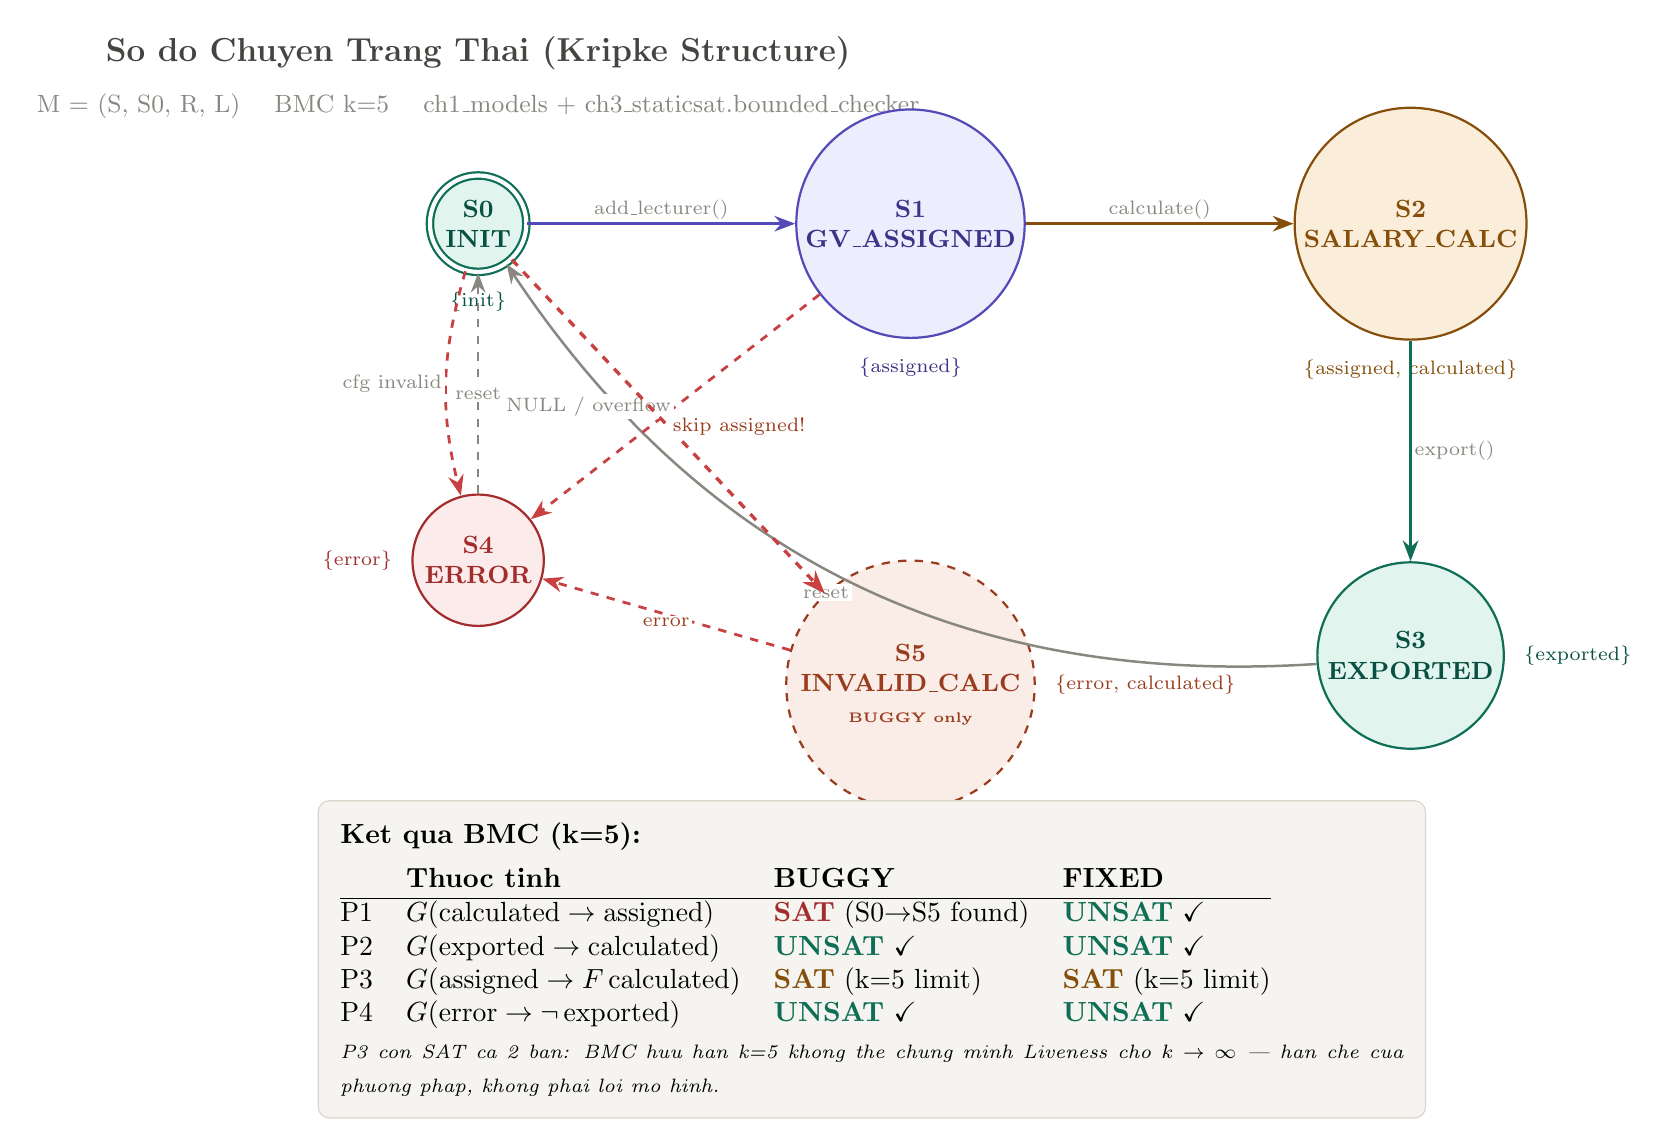
\begin{tikzpicture}[node distance=2.6cm and 3.0cm]

%% Title
\node[title main] (T1) at (0, 0)
  {So do Chuyen Trang Thai (Kripke Structure)};
\node[title sub, below=0.05cm of T1]
  {M = (S, S0, R, L) \quad BMC k=5 \quad
   ch1\_models + ch3\_staticsat.bounded\_checker};

%% --- STATES ---
\node[state init, below=1.2cm of T1] (S0)
  {S0\\INIT};

\node[state assigned, right=3.4cm of S0] (S1)
  {S1\\GV\_ASSIGNED};

\node[state calc, right=3.4cm of S1] (S2)
  {S2\\SALARY\_CALC};

\node[state exported, below=2.8cm of S2] (S3)
  {S3\\EXPORTED};

\node[state error, below=2.8cm of S0] (S4)
  {S4\\ERROR};

%% S5 — BUGGY only
\node[state buggy, below=2.8cm of S1] (S5)
  {S5\\INVALID\_CALC\\{\tiny BUGGY only}};

%% --- LABELS ---
\node[font=\scriptsize, text=CTeal800, below=0.12cm of S0]
  {\{init\}};
\node[font=\scriptsize, text=CPurple800, below=0.12cm of S1]
  {\{assigned\}};
\node[font=\scriptsize, text=CAmber600, below=0.12cm of S2]
  {\{assigned, calculated\}};
\node[font=\scriptsize, text=CTeal800, right=0.12cm of S3]
  {\{exported\}};
\node[font=\scriptsize, text=CRed600, left=0.12cm of S4]
  {\{error\}};
\node[font=\scriptsize, text=CCoral600, right=0.12cm of S5]
  {\{error, calculated\}};

%% --- TRANSITIONS FIXED ---
%% S0 -> S1
\draw[arr purple]
  (S0) -- node[edge label, above] {add\_lecturer()} (S1);
%% S1 -> S2
\draw[arr amber]
  (S1) -- node[edge label, above] {calculate()} (S2);
%% S2 -> S3
\draw[arr teal]
  (S2) -- node[edge label, right] {export()} (S3);
%% S3 -> S0 (reset)
\draw[arr, bend left=30]
  (S3) to node[edge label, below left] {reset} (S0);
%% S1 -> S4 (error)
\draw[arr red]
  (S1) -- node[edge label, left] {NULL / overflow} (S4);
%% S4 -> S0
\draw[arr, dashed]
  (S4) -- node[edge label, below] {reset} (S0);
%% S0 -> S4 (direct error)
\draw[arr red, bend right=15]
  (S0) to node[edge label, left] {cfg invalid} (S4);

%% --- S5 BUGGY PATH ---
\draw[arr red, dashed, very thick]
  (S0) -- node[edge label, right, text=CCoral600]
    {skip assigned!} (S5);
\draw[arr red, dashed]
  (S5) -- node[edge label, below, text=CCoral600] {error} (S4);

%% --- BMC RESULTS BOX ---
\node[draw=CGray200, fill=CGray50, rounded corners=4pt,
  inner sep=8pt, below=2.2cm of S4, xshift=5cm] (bmc box)
{
  \parbox{13.5cm}{
    \textbf{Ket qua BMC (k=5):}\\[4pt]
    \begin{tabular}{@{}llll@{}}
      & \textbf{Thuoc tinh} & \textbf{BUGGY} & \textbf{FIXED}\\
      \hline
      P1 & $G(\text{calculated}\to\text{assigned})$
         & \textcolor{CRed600}{\textbf{SAT}} (S0$\to$S5 found)
         & \textcolor{CTeal600}{\textbf{UNSAT}} $\checkmark$\\
      P2 & $G(\text{exported}\to\text{calculated})$
         & \textcolor{CTeal600}{\textbf{UNSAT}} $\checkmark$
         & \textcolor{CTeal600}{\textbf{UNSAT}} $\checkmark$\\
      P3 & $G(\text{assigned}\to F\,\text{calculated})$
         & \textcolor{CAmber600}{\textbf{SAT}} (k=5 limit)
         & \textcolor{CAmber600}{\textbf{SAT}} (k=5 limit)\\
      P4 & $G(\text{error}\to\neg\,\text{exported})$
         & \textcolor{CTeal600}{\textbf{UNSAT}} $\checkmark$
         & \textcolor{CTeal600}{\textbf{UNSAT}} $\checkmark$\\
    \end{tabular}\\[4pt]
    \textit{\scriptsize P3 con SAT ca 2 ban: BMC huu han k=5 khong the chung minh Liveness cho $k\to\infty$ --- han che cua phuong phap, khong phai loi mo hinh.}
  }
};

\end{tikzpicture}
\end{document}
